Given the learned parameters and a new
observation sequence $x = x_1\ldots x_N$, we want to find the sequence of hidden states $y^* = y_1^* \ldots y_N^*$ that ``best'' explains it.
 This is called the \emph{decoding} problem. There are several ways to define what we mean by the ``best''
$y^*$, depending on our goal: for instance, we may want to minimize the probability of error
on each hidden
variable $Y_i$, or we may want to find the best assignment
to the sequence $Y_1\ldots Y_N$ as a whole. 
Therefore, finding the best sequence
can be accomplished through different approaches:

\begin{itemize}
\item A first approach, normally called \textbf{posterior decoding} or \textbf{minimum risk decoding}, consists
in picking the highest state posterior for each position $i$ in the sequence:
\begin{equation}
y_i^* = \argmax_{y_i \in \Lambda} P(Y_i=y_i | X_1=x_1,\ldots,X_N =x_N).
\end{equation}
%where $\gamma_i(\hs_i)$ is the posterior probability $P(\hs_i|\sent)$. 
Note, however, that this approach does not guarantee that the sequence $y^*=y_1^* \ldots y_N^*$ will be a
valid sequence of the model. For instance, there might be a transition
between two of the best state posteriors with probability zero. 

\item A second approach, called \textbf{Viterbi decoding}, consists in
picking the best global hidden state sequence: 
\begin{eqnarray}
y^* &=& \argmax_{y = y_1\ldots y_N} P(Y_1=y_1,\ldots, Y_N=y_N | X_1=x_1,\ldots,X_N =x_N)\nonumber\\
&=& \argmax_{y = y_1\ldots y_N} P(Y_1=y_1,\ldots, Y_N=y_N, X_1=x_1,\ldots,X_N =x_N).
\end{eqnarray}
\end{itemize}

Both approaches (which will be explained in Sections~\ref{posterior} and~\ref{viterbi}, respectively) rely on dynamic programming and make use of the
independence assumptions of the HMM model. Moreover, they use an alternative
representation of the HMM called a \emph{trellis}. 

A trellis unfolds all possible states for each position and it makes explicit the independence assumption: each position only
depends on the previous position. Here, each column represents a position in the sequence and each row represents a possible state. Figure \ref{fig:trellis} shows the
trellis for the particular example in Figure \ref{fig:hmm}. 

\begin{figure}[ht]
\centering
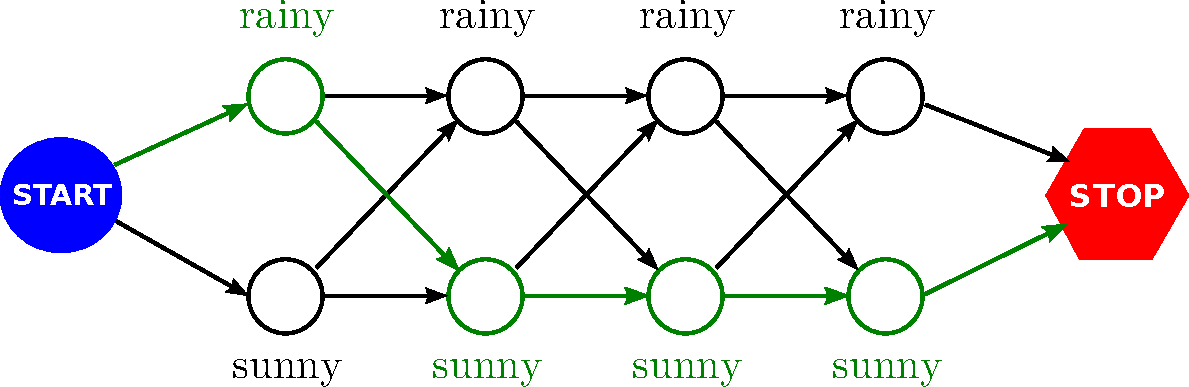
\includegraphics[width=0.7\textwidth]{figs/sequences/trellis_new}
\caption[HMM Trellis representation.]{\label{fig:trellis} Trellis
  representation of the HMM in Figure ~\ref{fig:hmm}, for the observation
  sequence ``{\tt walk} {\tt walk} {\tt shop} {\tt clean}'', where each hidden variable can take the values {\tt rainy} or {\tt sunny}.}
\end{figure}




Considering the trellis representation, note that we can include the following information:
\begin{itemize}
\item an \emph{initial probability} to the arrows that depart from the start symbol;
\item a \emph{final probability} to the arrows that reach the stop symbol;
\item a \emph{transition probability} to the remaining arrows; and,
\item an \emph{emission probability} to each circle, which is the probability that the observed symbol is emitted by that particular state.
\end{itemize}

For convenience, we will be working with 
log-probabilities, rather than probabilities.\footnote{This will be motivated further in Section~\ref{sec:logdomain}, where we describe 
how operations can be performed efficiently
in the log-domain.} Therefore, if we associate to each circle and arrow in
the trellis a score that corresponds
to the log-probabilities above, 
and if we define the score of a path
connecting the {\tt start} and  {\tt stop} symbols as
the sum of the scores of the circles and arrows
it traverses, 
then 
the goal of finding the most likely sequence of states (Viterbi decoding) corresponds to 
finding the path with the highest score.




%---since 
%we'll be multiplying a lot of probabilities, 
%we prevent underflowing by working in the log-domain. 

%For the decoding algorithms described in the following sections, 
%it is
%useful to define a re-parametrization of the model in equation \eqref{eqn:hmm}, in terms of
%node potentials $\phi_n(l)$ (associating a number to each box in Figure \ref{fig:trellis})
%and edge potentials $\phi_{n-1,n}(l,m)$ (associating a number to each edge in  Figure
%\ref{fig:trellis}). For our example, this re-parametrization is given by
%%
%\begin{equation}
%  \joint =\phi_1(r)\phi_1(r,s)\phi_2(s)\phi_2(s,s)\phi_3(s)\phi_3(s,s)\phi_4(s).
%  \label{eqn:hmm_ex_treelis}
%\end{equation}
%
%%\begin{equation}
%%  \joint =\phi_1(``w'',r)\phi_1(r,s)\phi_2(``w'',s)\phi_2(s,s)\phi_3(``s'',s)\phi_3(s,s)\phi_4(``c'',s).
%%  \label{eqn:hmm_ex_treelis}
%%\end{equation}
%
%In other words, to do this re-parameterization we need to find expressions for the potential variables, (the $\phi$'s) such that \eqref{eqn:hmm} and \eqref{eqn:hmm_ex_treelis} are equal. The solution is given by
%\begin{equation}
%\phi_{i-1,i}(l,m) = a_{l,m}
%\label{eq:nodes1}
%\end{equation}
%and
%\begin{equation}
%\phi_i(l) = 
%\begin{cases}
% b_{\obs_i}(l)\pi_l \quad\text{i = 1}\\
% b_{\obs_i}(l) \quad\text{i = 2,\ldots,N-1}\\
% b_{\obs_i}(l)a_{l,STOP} \quad\text{i = N}
% \label{eq:nodes2}
%\end{cases}
%\end{equation}


%\begin{itemize}
%\item\emph{Edge Potentials} - correspond to the transition parameters, with the exception of the
%edges into the last position that correspond to the final transition parameters.
%\item\emph{Node Potentials} - correspond to the observation
%parameters for a given state and the observation at that position.  The
%first position is the exception and corresponds to the
%product between the observation parameters for that state and
%the observation in that position with the initial parameters for that state. 
%\end{itemize}

%Although this re-parametrization simplifies the exposition, and will be
%used in these lectures, it is not necessarily very practical since we
%will be reproducing several values (for instance the transition
%parameters for each position).


The trellis scores are given by the following expressions:
\begin{itemize}
\item For each state $c_k$:
\begin{eqnarray}
\mathrm{score}_{\mathrm{init}}(c_k) &=&
\log P_{\mathrm{init}}(Y_{1} = c_k | \text{\tt start}).
\end{eqnarray}
\item For each position $i \in {1,\ldots,N-1}$ and each pair of states $c_k$ and $c_l$:
\begin{eqnarray}
\mathrm{score}_{\mathrm{trans}}(i, c_k, c_l) &=&
\log P_{\mathrm{trans}}(Y_{i+1} = c_k | Y_i = c_l).
\end{eqnarray}
\item For each state $c_l$:
\begin{eqnarray}
\mathrm{score}_{\mathrm{final}}(c_l) &=&
\log P_{\mathrm{final}}(\text{\tt stop} | Y_N = c_l).
\end{eqnarray}
\item For each position $i \in {1,\ldots,N}$ and state $c_k$:
\begin{eqnarray}
\mathrm{score}_{\mathrm{emiss}}(i, c_k) &=&
\log P_{\mathrm{emiss}}(X_i = x_i | Y_i = c_k).
\end{eqnarray}
\end{itemize}

In the next exercise, you will compute the trellis scores.

\begin{exercise}
Convince yourself that the score of a path in the trellis 
(summing over the scores above) is equivalent 
to the log-probability $\log P(X=x,Y=y)$, 
as defined in 
Eq.~\ref{eqn:hmm_ex}. 
Use the given function \emph{compute\_scores} on the first training sequence and confirm that the values are correct. You should get the same values as presented below.

%Implement a function that builds the node and edge potentials for a
%given sequence. The function head is in the \emph{hmm.py} file:

%\begin{python}
% def build_potentials(self,sequence):
%\end{python}
%
%Run this function for the first training sequence from the simple
%dataset and compare the results given (If the results are the same
%then you are ready to go).

\begin{python}
>>> initial_scores, transition_scores, final_scores, emission_scores = hmm.compute_scores(simple.train.seq_list[0])
>>> print initial_scores
[-0.40546511 -1.09861229]
>>> print transition_scores
[[[-0.69314718        -inf]
  [-0.69314718 -0.47000363]]

 [[-0.69314718        -inf]
  [-0.69314718 -0.47000363]]

 [[-0.69314718        -inf]
  [-0.69314718 -0.47000363]]]
>>> print final_scores
[       -inf -0.98082925]
>>> print emission_scores
[[-0.28768207 -1.38629436]
 [-0.28768207 -1.38629436]
 [-1.38629436 -0.98082925]
 [       -inf -0.98082925]] 
\end{python}

Note that scores which are $-\infty$ (\texttt{-inf}) correspond
to zero-probability events. 
\end{exercise}

\subsection{Computing in log-domain}\label{sec:logdomain}

We will see that the decoding algorithms 
will need to multiply twice as many probability terms as 
the length $N$ of the sequence. 
This may cause underflowing problems 
when $N$ is large, since the nested multiplication of numbers smaller than 1
may easily become smaller than the machine precision. To avoid that
problem, \cite{rabiner} presents a scaled version of the decoding algorithms that avoids this problem.
An alternative, which is widely used, is computing
in the log-domain. That is, instead of 
manipulating probabilities, manipulate log-probabilities (the scores presented above). 
Every time we need to multiply probabilities, 
we can sum their log-representations, since:
\begin{equation}
\log(\exp(a) \times \exp(b)) = a+b.
\end{equation}
Sometimes, we need to \emph{add} probabilities. 
In the log domain, this requires us to compute 
\begin{equation}
\log(\exp(a) + \exp(b)) = a + \log(1 + \exp(b-a)),
\end{equation}
where we assume that $a$ is smaller than $b$.


\begin{exercise}
Look at the module {\tt sequences/log\_domain.py}. 
This module implements a function
{\tt logsum\_pair(logx, logy)} to 
add two numbers represented in the log-domain;
it returns their sum also represented in the log-domain. The function {\tt logsum(logv)} 
sums all components of an array 
represented in the log-domain. 
This will be used later in our decoding algorithms.
To observe why this is important, type the 
following:
\begin{python}
>>> import numpy as np
>>> a = np.random.rand(10)
>>> np.log(sum(np.exp(a)))
2.8397172643228661
>>> np.log(sum(np.exp(10*a)))
10.121099917705818
>>> np.log(sum(np.exp(100*a)))
93.159220940569128
>>> np.log(sum(np.exp(1000*a)))
inf
>>> from lxmls.sequences.log_domain import *
>>> logsum(a)
2.8397172643228665
>>> logsum(10*a)
10.121099917705818
>>> logsum(100*a)
93.159220940569114
>>> logsum(1000*a)
925.88496219586864
\end{python}
\end{exercise}


\subsection{Posterior Decoding}\label{posterior}
Posterior decoding consists
in picking state with the highest posterior for each position in the sequence independently; for 
each $i = 1,\ldots,N$:
\begin{equation}
y_i^* = \argmax_{y_i \in \statevocab} P(Y_i=y_i | X = x).
\end{equation}
The \textbf{sequence posterior distribution} is the probability of a particular
hidden state sequence given that we have observed a particular
sequence. Moreover, we will be interested in two other posteriors distributions:
the \textbf{state posterior distribution}, corresponding to the
probability of being in a given state in a certain position given the
observed sequence; and the \textbf{transition posterior distribution},
which is the probability of making a particular transition, from position $i$ to
$i+1$, given the observed sequence. They are formally defined as follows:
\begin{align}
  \mathbf{Sequence \ Posterior\!:}\;\;\;\; &P(Y=y|X=x) = \frac{P(X=x,Y=y)}{P(X=x)}; \label{eq::posteriorDistribution} \\
 \mathbf{State \ Posterior\!:}\;\;\;\;  & P(Y_i=y_i | X=x); \label{eq::nodePosterior} \\
 \mathbf{Transition \ Posterior\!:}\;\;\;\;  &P(Y_{i+1}=y_{i+1},Y_i=y_i| X=x).\label{eq::edgePosterior}
\end{align}

To compute the posteriors, a first step is to be able to compute the 
likelihood of
the sequence $P(X=x)$, which corresponds to summing the probability of all
possible hidden state sequences.
\begin{equation}
\label{likelihoood}
\mathbf{Likelihood\!:}\;\;\;\; P(X=x) = \displaystyle \sum_{y \in \statevocab^N} P(X=x,Y=y).
\end{equation}
The number of possible hidden state sequences is exponential in the
length of the sequence ($|\statevocab|^N$),
 which makes the sum over all of them hard. 
 In our simple
 example, there are $2^4 = 16$ paths, which we can actually explicitly enumerate
 and calculate their probability using Equation \ref{eqn:hmm}. But this is as far as it goes: for example, for Part-of-Speech
 tagging with a small tagset of 12 tags and a medium size
 sentence of length 10, there are $12^{10} = 61 917 364 224$ such
 paths. 
Yet, we must be able to compute this sum (sum over $y \in \statevocab^N$) to compute the above likelihood
formula; this is called the inference problem. For sequence models, there is a well known dynamic programming algorithm,
the \textbf{Forward-Backward} (FB) algorithm, which allows the computation
to be performed in linear time,%
\footnote{The runtime is linear with respect
to the sequence length. More precisely, 
the runtime is $O(N|\statevocab|^2)$. 
A naive enumeration would cost $O(|\statevocab|^N)$.} %
by making use of the independence assumptions.

The FB algorithm relies on the independence of previous states
assumption, which  
is illustrated in the trellis view by having arrows only between consecutive states. 
The FB algorithm defines two auxiliary probabilities, the forward probability and the backward probability. 
\begin{equation}
\label{eq::forward}
\mathbf{Forward \ Probability\!:}\;\;\;\;  \mathrm{forward}(i, c_k) = P(Y_i = c_k, X_1=x_1,\ldots, X_i = x_i)
\end{equation}
The forward probability represents the probability that in position
$i$ we are in state $Y_i = c_k$ and that we have observed $x_1,\ldots,x_i$
up to that position. The forward probability is defined by the
following recurrence rule: 
\begin{eqnarray}
\mathrm{forward}(1, c_k) &=& P_{\mathrm{init}}(c_k|\text{\tt start}) \times 
P_{\mathrm{emiss}}(x_1 | c_k)
 \\
 \mathrm{forward}(i, c_k) &=& \left( \displaystyle \sum_{c_l \in \statevocab} P_{\mathrm{trans}}(c_k | c_l) \times \mathrm{forward}(i-1, c_l) \right) \times P_{\mathrm{emiss}}(x_i | c_k)  \label{forwardRecursion}
 \\
  \mathrm{forward}(N+1, \text{\tt stop}) &=& \sum_{c_l \in \statevocab} P_{\mathrm{final}}(\text{\tt stop} | c_l) \times \mathrm{forward}(N, c_l).
\end{eqnarray}

%\begin{figure}
%\begin{center}
%\begin{tabular}{cc}
%
%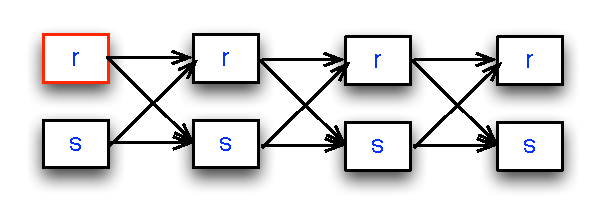
\includegraphics[scale=.5]{figs/sequences/forward1}
%& 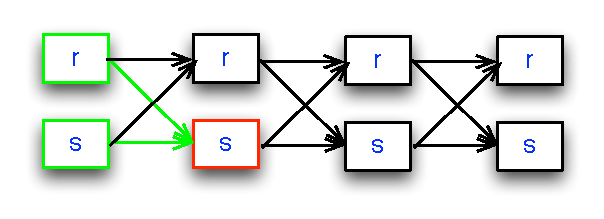
\includegraphics[scale=.5]{figs/sequences/forward2}\\
%\end{tabular}
%\caption[Forward-backward example.]{\label{fig:fb} Forward trellis for
%  the first sentence of the training data at position 1 (left) and at
%  position 2 (right)}
%
%\end{center}
%\end{figure}

%At position 1, the probability of being in state ``r'' and observing word ``w'' is just the node
%marginal for that position: $\alpha_1(r) = \phi_1(r)$ (see Figure
% \ref{fig:fb} left). At position 2 the probability
%of being in state ``s'' and observing the sequence of words ``w w''
%corresponds to the sum of all possible ways of reaching position 2 in
%state ``s'', namely, ``rs'' and ``ss'' (see Figure \ref{fig:fb} right). The probability of the former is
%$\phi_1(r)\phi_1(r,s)\phi_2(s)$
%and that of the latter is $\phi_1(s)\phi_1(s,s)\phi_2(s)$, so we get:
%\begin{eqnarray*}
%   \alpha_2(s) &=& \phi_1(r)\phi_1(r,s)\phi_2(s) +
%   \phi_1(s)\phi_1(s,s)\phi_2(s) \\
%   \alpha_2(s) &=& \left[\phi_1(r)\phi_1(r,s) +
%   \phi_1(s)\phi_1(s,s) \right]\phi_2(s) \\
% \alpha_2(s) &=& \displaystyle \sum_{\hs \in \hvocab}
% \left[\phi_1(\hs)\phi_1(\hs,s)\phi_2(s) \right] \\
%  \alpha_2(s) &=& \displaystyle \sum_{\hs \in \hvocab}
% \left[\alpha_1(\hs)\phi_1(\hs,s)\phi_2(s) \right]
%\end{eqnarray*}

Using the forward trellis one can compute the likelihood simply as:
\begin{equation}
\label{eq:forwardSum}
P(X=x) = \mathrm{forward}(N+1, \text{\tt stop}).
\end{equation}

Although the forward probability is enough to calculate the likelihood
of a given sequence, we will also need the backward probability to
calculate the state posteriors. 
The backward probability is similar to the forward probability, but operates in the inverse direction.
It 
represents the probability of observing $x_{i+1},\ldots,x_N$ from position $i+1$ up to $N$, given that at position $i$ we are at state $Y_i = c_l$:
 \begin{equation}
\label{eq::backward}
\mathbf{Backward \ Probability\!:}\;\;\;\;  \mathrm{backward}(i, c_l) = P(X_{i+1}=x_{i+1},\ldots, X_N=x_N | Y_i = c_l).
\end{equation}
The backward recurrence is given by:
\begin{eqnarray}
\mathrm{backward}(N, c_l) &=& P_{\mathrm{final}}(\text{\tt stop} | c_l) 
 \\
 \mathrm{backward}(i, c_l) &=&  \displaystyle \sum_{c_k \in \statevocab} P_{\mathrm{trans}}(c_k | c_l) \times \mathrm{backward}(i+1, c_k) \times P_{\mathrm{emiss}}(x_{i+1} | c_k)  \label{backwardRecursion}
 \\
  \mathrm{backward}(0, \text{\tt start}) &=& \sum_{c_k \in \statevocab} P_{\mathrm{init}}(c_k | \text{\tt start}) \times \mathrm{backward}(1, c_k) \times P_{\mathrm{emiss}}(x_{1} | c_k).
\end{eqnarray}
%At position $N$ there are no more observations, and the backward
%probability is set to 1. At position $i$, the probability 
%of having observed the future and being in state $\hv_l$, is given by the sum for all possible states of the probability of having transitioned 
%from position $i$ with state $\hv_l$ to position $i+1$ with state $\hv_m$, and observing $\obs_{i+1}$ at time $i+1$ and the future from there onward, which is $\beta_{i+1}(\hs_{i+1} = \hv_m)$. 
Using the backward trellis one can compute the likelihood simply as:.
\begin{equation}
\label{eq:backwardSum}
P(X=x) = \mathrm{backward}(0, \text{\tt start}).
\end{equation}
Moreover, with the forward and backward 
probabilities, we can compute the likelihood of a given sequence using any position $i$ in the sequence
as follows:
\begin{eqnarray}
\label{eq::fbsanity}
  P(X=x) &=& 
  \sum_{c_k \in \statevocab} P(X_1=x_1,\ldots, X_N=x_N,Y_i=c_k)\nonumber\\
  &=&
  \sum_{c_k \in \statevocab} 
  \underbrace{P(X_1=x_1,\ldots, X_i=x_i, Y_i=c_k)}_{\mathrm{forward}(i,c_k)} \times 
  \underbrace{P(X_{i+1}=x_{i+1},\ldots, X_N=x_N| Y_i=c_k)}_{\mathrm{backward}(i,c_k)}\nonumber\\
  &=& \sum_{c_k \in \statevocab} \mathrm{forward}(i,c_k) \times \mathrm{backward}(i,c_k).
\end{eqnarray}

This equation will work for any choice of $i$. Although redundant, this fact is useful when implementing an
HMM as a sanity check that the computations are being performed
correctly, since one can compute this expression for several $i$; they should all yield the same value. 

Algorithm \ref{alg:fb} shows the pseudo code for the forward backward algorithm.



\begin{algorithm}[t]
   \caption{Forward-Backward algorithm \label{alg:fb}}
\begin{algorithmic}[1]
   \STATE {\bfseries input:} sequence $x_1,\ldots,x_N$, scores $P_{\mathrm{init}}, P_{\mathrm{trans}}, P_{\mathrm{final}}, P_{\mathrm{emiss}}$
        \STATE  \emph{Forward pass}: Compute the forward probabilities
        \STATE \emph{Initialization}
        \FOR{$c_k \in \statevocab$ }
        \STATE $\mathrm{forward}(1,c_k) = P_{\mathrm{init}}(c_k|\text{\tt start}) \times 
P_{\mathrm{emiss}}(x_1 | c_k)$
        \ENDFOR 
        \FOR{$i=2$ {\bfseries to} $N$}
         \FOR{$c_k \in \statevocab$ }
                 \STATE $\mathrm{forward}(i, c_k) = \left( \displaystyle \sum_{c_l \in \statevocab} P_{\mathrm{trans}}(c_k | c_l) \times \mathrm{forward}(i-1, c_l) \right) \times P_{\mathrm{emiss}}(x_i | c_k)$
         \ENDFOR 
        \ENDFOR 
       \STATE \emph{Backward pass}: Compute the backward probabilities
       \STATE \emph{Initialization}
        \FOR{$c_l \in \statevocab$ }
        \STATE $\mathrm{backward}(N, c_l) = P_{\mathrm{final}}(\text{\tt stop} | c_l)$
        \ENDFOR 
       \FOR{$i=N-1$ {\bfseries to} 1}
        \STATE $\mathrm{backward}(i, c_l) =  \displaystyle \sum_{c_k \in \statevocab} P_{\mathrm{trans}}(c_k | c_l) \times \mathrm{backward}(i+1, c_k) \times P_{\mathrm{emiss}}(x_{i+1} | c_k)$
        \ENDFOR 
       \STATE \textbf{output:} The forward and backward probabilities.
\end{algorithmic}
\end{algorithm}





\begin{exercise}
%Given the implementation of the forward pass of the forward backward
%algorithm in the file \emph{forward\_backward.py}, implement the backward pass.
%\begin{python}
%
%def forward_backward(node_potentials,edge_potentials):
%    H,N = node_potentials.shape
%    forward = np.zeros([H,N],dtype=float)
%    backward = np.zeros([H,N],dtype=float)
%    forward[:,0] = node_potentials[:,0]
%    ## Forward loop
%    for pos in xrange(1,N):
%        for current_state in xrange(H):
%            for prev_state in xrange(H):
%                forward_v = forward[prev_state,pos-1]
%                trans_v = edge_potentials[prev_state,current_state,pos-1]
%                prob = forward_v*trans_v
%                forward[current_state,pos] += prob
%            forward[current_state,pos] *= node_potentials[current_state,pos]
%    ## Backward loop
%          ## Your code
%   return forward,backward
%
%\end{python}

Run the provided forward-backward algorithm on the first train sequence. 
Observe that both the forward and the backward 
passes give the same log-likelihood.
%Use the provided function that makes use of Equation \ref{eq::fbsanity} to make
%sure your implementation is correct: 
\begin{python}
>>> log_likelihood, forward = hmm.decoder.run_forward(initial_scores, transition_scores, final_scores, emission_scores)
>>> print 'Log-Likelihood =', log_likelihood
Log-Likelihood = -5.06823232601
>>> log_likelihood, backward = hmm.decoder.run_backward(initial_scores, transition_scores, final_scores, emission_scores)
>>> print 'Log-Likelihood =', log_likelihood
Log-Likelihood = -5.06823232601
\end{python}
\end{exercise}


Given the forward and backward probabilities, one can compute both the state
and transition posteriors 
(you can hint why by looking at the term inside the sum in Eq.~\ref{eq::fbsanity}).


\begin{align}
 \mathbf{State \ Posterior\!:}\;\;\;\;  & P(Y_i = y_i| X=x) = \frac{\mathrm{forward}(i, y_i) \times 
 \mathrm{backward}(i, y_i)}{P(X=x)}; \label{eq::nodePosterior2} \\
 \mathbf{Transition \ Posterior\!:}\;\;\;\; &
 P(Y_i = y_i, Y_{i+1} = y_{i+1} | X=x)= \nonumber\\
 &
   \frac{\mathrm{forward}(i, y_i) \times 
   P_{\mathrm{trans}}(y_{i+1}|y_i) \times
   P_{\mathrm{emiss}}(x_{i+1}|y_{i+1}) \times
 \mathrm{backward}(i+1, y_{i+1})}{P(X=x)}.\label{eq::edgePosterior2}
\end{align}

A graphical representation of these posteriors is illustrated in Figure~\ref{fig:posteriors}. 
On the left it is shown that $\mathrm{forward}(i, y_i)  \times \mathrm{backward}(i, y_i)$ returns the sum of all paths that contain the state $y_i$, weighted by $P(X=x)$; on the right we can see that $\mathrm{forward}(i, y_i) \times P_{\mathrm{trans}}(y_{i+1}|y_i) \times P_{\mathrm{emiss}}(x_{i+1}|y_{i+1}) \times \mathrm{backward}(i+1, y_{i+1})$  returns the same for all paths containing the edge from $y_i$ to $y_{i+1}$.
%Thus, these posteriors can be seen as the ratio of the number of paths that contain the given state or transition (weighted by $P(X=x)$) and the number of possible paths in the graph $\marginal$.

As a practical example, given that the person performs the sequence of actions ``{\tt walk} {\tt walk} {\tt shop} {\tt clean}", we want to know the probability of having been raining in the second day. The state posterior probability for this event can be seen as the probability that the sequence of actions above was generated by a sequence of weathers and where it was raining in the second day. In this case, the possible sequences would be all the sequences which have {\tt rainy} in the second position.

\begin{figure}
\begin{center}
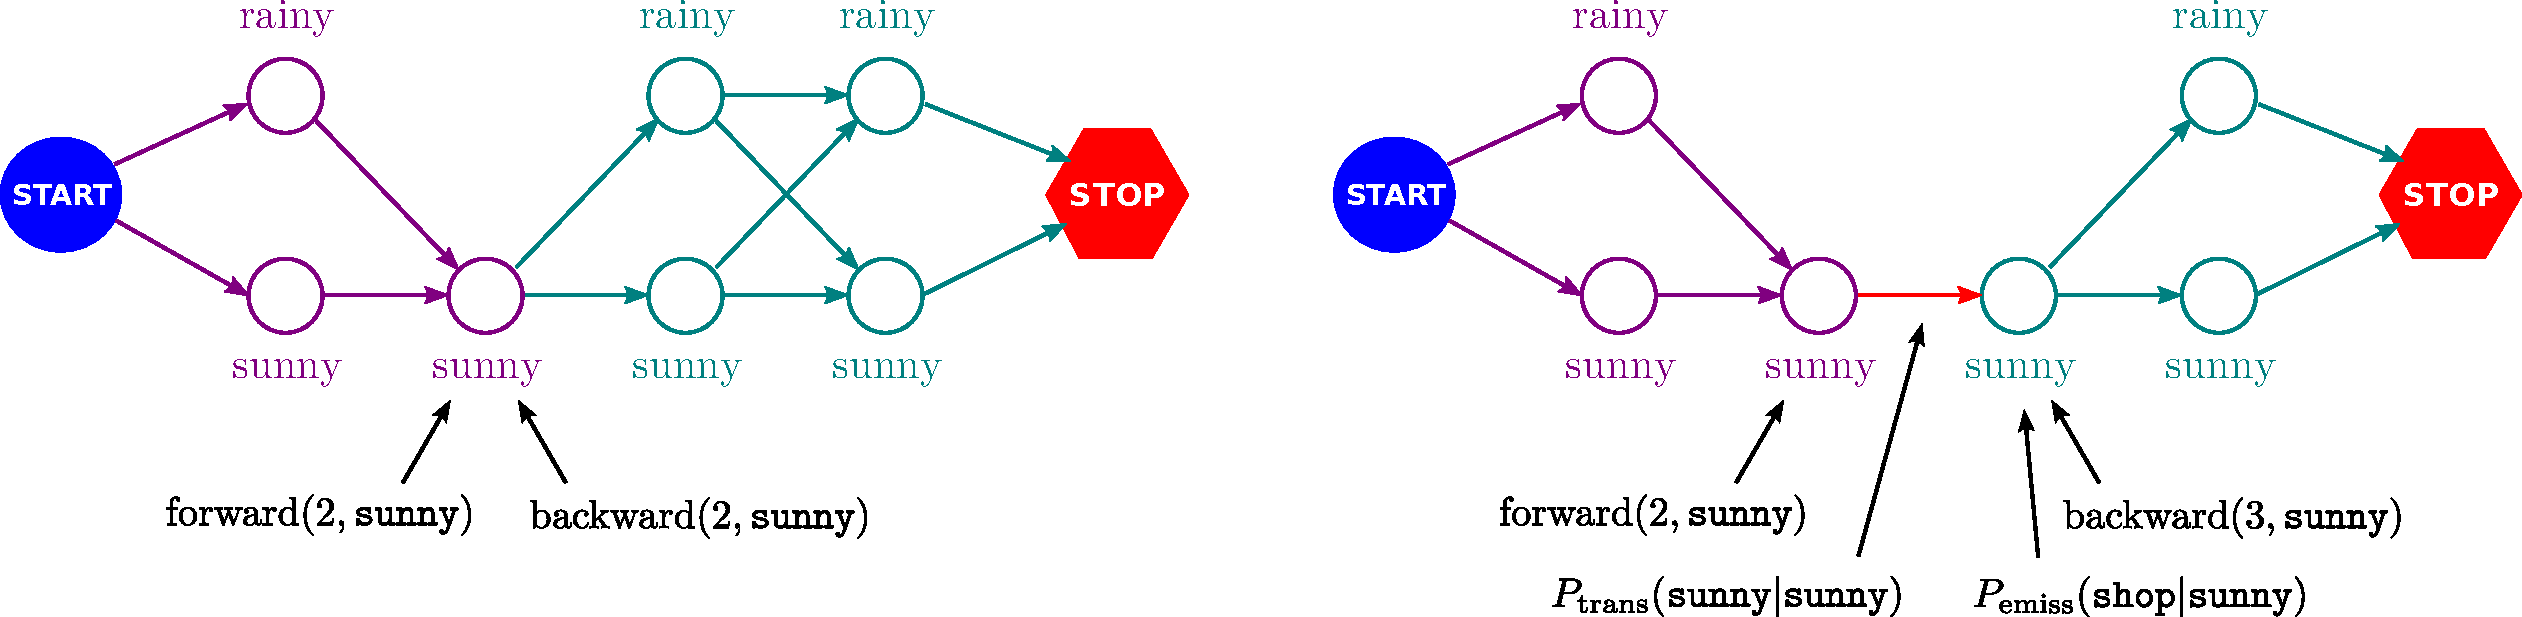
\includegraphics[width=1\textwidth]{figs/sequences/posteriors}
\caption[Posterior Illustration.]{\label{fig:posteriors} A graphical representation of the components in the state and transition posteriors. Recall that the observation sequence is ``\texttt{walk walk shop clean}''.}
\end{center}
\end{figure}

%\begin{figure}
%\begin{center}
%\begin{tabular}{cc}
%
%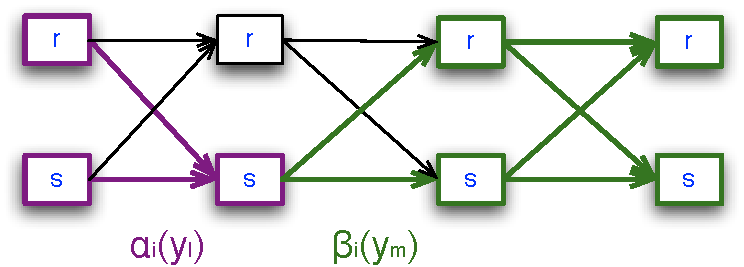
\includegraphics[scale=.5]{figs/sequences/statePost}
%& 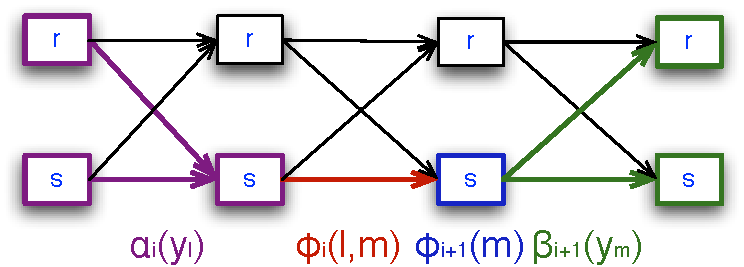
\includegraphics[scale=.5]{figs/sequences/transPost}\\
%\end{tabular}
%\caption[Posterior Illustration.]{\label{fig:posteriors} A graphical representation of the components in the state and transition posteriors.}
%
%\end{center}
%\end{figure}

Using the state posteriors, we are ready to perform posterior
decoding. 
The strategy is to compute the state posteriors 
for each position $i \in \{1,\ldots,N\}$
and each state $c_k \in \statevocab$, and 
then pick the arg-max at each position:
\begin{equation}
{\widehat y_i} := \argmax_{y_i \in \statevocab} P(Y_i=y_i| X=x).
\end{equation}

%Algorithm \ref{alg:pd} shows the posterior decoding algorithm.

%\begin{algorithm}[t]
%   \caption{Posterior Decoding algorithm \label{alg:pd}}
%\begin{algorithmic}[1]
%   \STATE {\bfseries input:} The forward and backward probabilities
%       $\alpha$ and $\beta$.
%   \STATE  \emph{Compute Likelihood}: Compute the likelihood of the
%   sentence
%   \STATE $L = 0$
%   \FOR{$\hv_l \in \hvocab$ }
%   \STATE $\marginal = \marginal + \alpha_N(\hv_l)$
%   \ENDFOR 
%   \STATE $\hat \hseq = []$
%    \FOR{$i=1$ {\bfseries to} $N$}
%    \STATE $max = 0$
%     \FOR{$\hv_l \in \hvocab$ }
%     \STATE $\gamma_i(\hv_l)  =  \frac{\alpha_i(\hv_l)
%       \beta_i(\hv_l)}{\marginal}$
%     \IF {$\gamma_i(\hv_l) > max$}
%     \STATE $max = \gamma_i(\hv_l)$
%     \STATE $\hat  y_i = \hv_l$
%     \ENDIF
%     \ENDFOR 
%     \ENDFOR 
%   \STATE \textbf{output:} the posterior path $\hat \hseq$
%\end{algorithmic}
%\end{algorithm}



\begin{exercise}
%Given the node and edge posterior formulas \ref{eq::nodePosterior},\ref{eq::edgePosterior} and the
%  forward and backward formulas \ref{eq::forward},\ref{eq::backward}, convince yourself that formulas
%  \ref{eq::nodePosterior2},\ref{eq::edgePosterior2} are correct. 

Compute the node posteriors for the first training sequence (use the provided \emph{compute\_posteriors} function), and look at
the output. Note that the state posteriors are a proper
probability distribution (the lines of the result sum to 1).

\begin{python}
>>> initial_scores, transition_scores, final_scores, emission_scores = hmm.compute_scores(simple.train.seq_list[0])
>>> state_posteriors, _, _ = hmm.compute_posteriors(initial_scores,
                                                    transition_scores,
                                                    final_scores,
                                                    emission_scores)
>>> print state_posteriors
[[ 0.95738152  0.04261848]
 [ 0.75281282  0.24718718]
 [ 0.26184794  0.73815206]
 [ 0.          1.        ]]
\end{python}
\end{exercise}

\begin{exercise}
Run the posterior decode on the first test sequence, and evaluate it.
\begin{python}
>>> y_pred = hmm.posterior_decode(simple.test.seq_list[0])
>>> print "Prediction test 0:", y_pred
walk/rainy walk/rainy shop/sunny clean/sunny
>>> print "Truth test 0:", simple.test.seq_list[0]
walk/rainy walk/sunny shop/sunny clean/sunny 
\end{python}

Do the same for the second test sequence:
\begin{python}
>>> y_pred = hmm.posterior_decode(simple.test.seq_list[1])
>>> print "Prediction test 1:", y_pred
clean/rainy walk/rainy tennis/rainy walk/rainy 
>>> print "Truth test 1:", simple.test.seq_list[1]
clean/sunny walk/sunny tennis/sunny walk/sunny 
\end{python}

What is wrong? Note the observations for the second test sequence: the
observation {\tt tennis} was never seen at training time, so the probability for
it will be zero (no matter what state). This will make all possible state
sequences have zero probability.
As seen in the previous lecture, this is a problem with generative
models, which can be corrected using smoothing (among other
options).

Change the \emph{train\_supervised} method to add smoothing:
\begin{python}
def train_supervised(self,sequence_list, smoothing):
\end{python}

Try, for example, adding 0.1 to all the counts, and repeating this exercise with that smoothing. What do you observe?
\begin{python}
>>> hmm.train_supervised(simple.train, smoothing=0.1)
>>> y_pred = hmm.posterior_decode(simple.test.seq_list[0])
>>> print "Prediction test 0 with smoothing:", y_pred
walk/rainy walk/rainy shop/sunny clean/sunny 
>>> print "Truth test 0:", simple.test.seq_list[0]
walk/rainy walk/sunny shop/sunny clean/sunny
>>> y_pred = hmm.posterior_decode(simple.test.seq_list[1])
>>> print "Prediction test 1 with smoothing:", y_pred
clean/sunny walk/sunny tennis/sunny walk/sunny 
>>> print "Truth test 1:", simple.test.seq_list[1]
clean/sunny walk/sunny tennis/sunny walk/sunny 
\end{python}
\end{exercise}

%Note that if you use smoothing when training, the sanity checks mentioned at the start of this chapter are no longer true. For example, the sum of all the transition counts is no longer equal to the number of tokens -- it is larger.

%\begin{exercise}
%Change the function you just created \emph{ def
%  sanity\_check\_counts(self,seq\_list):} to account for smoothing. Make
%sure it works properly.
%
%\begin{python}
%In []: run sequences/hmm.py
%In []: hmm = HMM(simple)
%In []: hmm.collect_counts_from_corpus(simple.train,smoothing=0.1)
%In []: hmm.sanity_check_counts(simple.train,smoothing=0.1)
%Init Counts match
%Final Counts match
%Transition Counts match
%Observations Counts match
%\end{python}
%\end{exercise}


\subsection{Viterbi Decoding}\label{viterbi}


\textbf{Viterbi decoding} consists in
picking the best global hidden state sequence 
$\widehat{y}$
as follows: 
\begin{equation}
\widehat{y} = \argmax_{y \in \statevocab^N} P(Y=y|X=x) = \argmax_{y \in \statevocab^N} P(X=x,Y=y).
\end{equation}

The Viterbi algorithm 
is very similar to the forward procedure of the FB algorithm,
making use of the same trellis structure to efficiently represent the exponential number of sequences without prohibitive computation costs. In fact, the only
difference from the forward-backward algorithm is in the recursion
\ref{forwardRecursion} where instead of \emph{summing} over all possible 
hidden states, we take their \emph{maximum}.

\begin{equation}
\label{eq::viterbi}
\mathbf{Viterbi }\;\;\;\;  \mathrm{viterbi}(i, y_i) = \max_{y_1...y_{i-1}} P(Y_1=y_1,\ldots Y_i = y_i , X_1=x_1,\ldots, X_i=x_i)
\end{equation}
The Viterbi trellis represents the path with maximum probability in
position
$i$ when we are in state $Y_i=y_i$ and that we have observed $x_1,\ldots,x_i$
up to that position. The Viterbi algorithm is defined by the
following recurrence: 
\begin{eqnarray}
\mathrm{viterbi}(1, c_k) &=& P_{\mathrm{init}}(c_k|\text{\tt start}) \times 
P_{\mathrm{emiss}}(x_1 | c_k)
 \\
 \mathrm{viterbi}(i, c_k) &=& \left( \displaystyle \max_{c_l \in \statevocab} P_{\mathrm{trans}}(c_k | c_l) \times \mathrm{viterbi}(i-1, c_l) \right) \times P_{\mathrm{emiss}}(x_i | c_k)  \label{viterbiRecursion}
 \\
 \mathrm{backtrack}(i, c_k) &=& \left( \displaystyle \argmax_{c_l \in \statevocab} P_{\mathrm{trans}}(c_k | c_l) \times \mathrm{viterbi}(i-1, c_l) \right) 
 \\
  \mathrm{viterbi}(N+1, \text{\tt stop}) &=& \max_{c_l \in \statevocab} P_{\mathrm{final}}(\text{\tt stop} | c_l) \times \mathrm{viterbi}(N, c_l)
 \\
  \mathrm{backtrack}(N+1, \text{\tt stop}) &=& \argmax_{c_l \in \statevocab} P_{\mathrm{final}}(\text{\tt stop} | c_l) \times \mathrm{viterbi}(N, c_l).
\end{eqnarray}


%\begin{eqnarray}
%\delta_1(\hv_l) &=& \phi_1(l) \\
%\delta_i(\hv_l) &=& \left[ \max_{y_1 ... y_i} \phi_{i-1,i}(m,l)
%  \delta_{i-1}(\hv_m) \right] \phi_i(l) \label{viterbiRecursion} \\
%\psi_{i}(\hv_l) &=& \left[ \argmax_{y_1 ... y_i} \phi_{i-1,i}(m,l)
%  \delta_{i-1}(\hv_m) \right]
%%\phi_{(i-1)}(m,l)  \delta_{i-1}(\hv_m) \right] \phi_i(l) \label{viterbiBackpointers}
%\end{eqnarray}

Algorithm \ref{alg:viterbi} shows the pseudo code for the Viterbi algorithm.
Note the similarity with the forward algorithm.
The only differences are:
\begin{itemize}
\item Maximizing instead of summing;
\item Keeping the argmax's to backtrack.
\end{itemize}

%\begin{algorithm}[t]
%   \caption{Viterbi algorithm \label{alg:viterbi}}
%\begin{algorithmic}[1]
%   \STATE {\bfseries input:} sentence $\sent$, parameters $\theta$
%        \STATE  \emph{Forward pass}: compute the maximum paths for
%        every end state
%        \STATE \emph{Initialization}
%        \FOR{$\hv_l \in \hvocab$ }
%        \STATE $\delta_1(\hv_l) = \phi_1(\hv_l)$
%        \ENDFOR 
%        \FOR{$i=2$ {\bfseries to} $N$}
%         \FOR{$\hv_l \in \hvocab$ }
%                 \STATE $\delta_i(\hv_l) = \left[ \displaystyle
%                   \max_{m  \in \hvocab} \phi_{i-1,i}(m,l)
%                   \delta_{i-1}(\hv_m) \right] \phi_i(l)$
%                 \STATE $\psi_{i}(\hv_l) = m$
%         \ENDFOR 
%        \ENDFOR 
%       %\STATE \emph{Terminate}:
%       \STATE 
%  $\max_{y \in \statevocab^N} P(X=x,Y=y) := \max_{c_l \in \statevocab} P_{\mathrm{final}}(\text{\tt stop} | c_l) \times \mathrm{viterbi}(N, c_l)$
%  	   \STATE 
%       \STATE \emph{Backward pass}: Build the most likely path
%	  \STATE $\widehat{y}_i = \argmax_{c_l \in \statevocab} P_{\mathrm{final}}(\text{\tt stop} | c_l) \times \mathrm{viterbi}(N, c_l)$ 
%	   \FOR{$i=N-1$ {\bfseries to} 1}
%        \STATE $\widehat{y_i} = \mathrm{backtrack}(i+1, \widehat{y}_{i+1})$
%        \ENDFOR 
%       \STATE \textbf{output:} the viterbi path $\widehat{y}$
%\end{algorithmic}
%\end{algorithm}

\begin{algorithm}[t]
   \caption{Viterbi algorithm \label{alg:viterbi}}
\begin{algorithmic}[1]
   \STATE {\bfseries input:} sequence $x_1,\ldots,x_N$, scores $P_{\mathrm{init}}, P_{\mathrm{trans}}, P_{\mathrm{final}}, P_{\mathrm{emiss}}$
        \STATE  \emph{Forward pass}: Compute the best paths for every end state
        \STATE \emph{Initialization}
        \FOR{$c_k \in \statevocab$ }
        \STATE $\mathrm{viterbi}(1,c_k) = P_{\mathrm{init}}(c_k|\text{\tt start}) \times 
P_{\mathrm{emiss}}(x_1 | c_k)$
        \ENDFOR 
        \FOR{$i=2$ {\bfseries to} $N$}
         \FOR{$c_k \in \statevocab$ }
          \STATE $\mathrm{viterbi}(i, c_k) = \left( \displaystyle \max_{c_l \in \statevocab} P_{\mathrm{trans}}(c_k | c_l) \times \mathrm{viterbi}(i-1, c_l) \right) \times P_{\mathrm{emiss}}(x_i | c_k)$
          \STATE $\mathrm{backtrack}(i, c_k) = \left( \displaystyle \argmax_{c_l \in \statevocab} P_{\mathrm{trans}}(c_k | c_l) \times \mathrm{viterbi}(i-1, c_l) \right)$
         \ENDFOR 
        \ENDFOR 
       \STATE 
  $\max_{y \in \statevocab^N} P(X=x,Y=y) := \max_{c_l \in \statevocab} P_{\mathrm{final}}(\text{\tt stop} | c_l) \times \mathrm{viterbi}(N, c_l)$        
        \STATE
       \STATE \emph{Backward pass}: backtrack to obtain the most likely path 
	  \STATE $\widehat{y}_N = \argmax_{c_l \in \statevocab} P_{\mathrm{final}}(\text{\tt stop} | c_l) \times \mathrm{viterbi}(N, c_l)$ 
	   \FOR{$i=N-1$ {\bfseries to} 1}
        \STATE $\widehat{y_i} = \mathrm{backtrack}(i+1, \widehat{y}_{i+1})$
        \ENDFOR 
       \STATE \textbf{output:} the viterbi path $\widehat{y}$.
\end{algorithmic}
\end{algorithm}

\section{Assignment}

With the previous theoretical background, you have the necessary tools to solve today's assignment.

\begin{exercise}
Implement a method 
for performing Viterbi decoding in 
file {\tt sequence\_classification\_decoder.py}.
\begin{python}
        def run_viterbi(self, initial_scores, transition_scores, final_scores, emission_scores):
\end{python}
Hint: look at the implementation of {\tt run\_forward}. Also check the help for the numpy methods max and argmax.

This method will be called 
by 
\begin{python}
def viterbi_decode(self, sequence)
\end{python}
in the module {\tt sequence\_classifier.py}.
%
%posterior decoding (the function \emph{posterior\_decode}) for reference.

Test your method on both test sequences and compare the results with
the ones given.
\begin{python}
>>> hmm.train_supervised(simple.train, smoothing=0.1)
>>> y_pred, score = hmm.viterbi_decode(simple.test.seq_list[0])
>>> print "Viterbi decoding Prediction test 0 with smoothing:", y_pred, score
walk/rainy walk/rainy shop/sunny clean/sunny  -6.02050124698
>>> print "Truth test 0:", simple.test.seq_list[0]
walk/rainy walk/sunny shop/sunny clean/sunny 
>>> y_pred, score = hmm.viterbi_decode(simple.test.seq_list[1])
>>> print "Viterbi decoding Prediction test 1 with 
smoothing:", y_pred, score
clean/sunny walk/sunny tennis/sunny walk/sunny  -11.713974074
>>> print "Truth test 1:", simple.test.seq_list[1]
clean/sunny walk/sunny tennis/sunny walk/sunny 
\end{python}

Note: since we didn't run the \emph{train\_supervised} method again, we are still using the result of the training using smoothing. Therefore, you should compare these results to the ones of posterior decoding with smoothing.

\end{exercise}




%%% Local Variables: 
%%% mode: latex
%%% TeX-master: "../../guide"
%%% End: 
